\documentclass{beamer}

\usetheme{Madrid} % Singapore, Madrid, Ilmenau, CambridgeUS
\setbeamertemplate{navigation symbols}{}

% --- Colores personalizados ---
\definecolor{unahurverde}{HTML}{005C5C}
\definecolor{unahurgris}{HTML}{EAEAEA}
\setbeamercolor{structure}{fg=unahurverde}
\setbeamercolor{frametitle}{bg=unahurverde, fg=white}
\setbeamercolor{title}{fg=unahurverde}
\setbeamercolor{block title}{bg=unahurverde, fg=white}
\setbeamercolor{block body}{bg=unahurgris, fg=black}

% --- Logo en esquina superior derecha ---
\addtobeamertemplate{frametitle}{}{%
	\begin{textblock*}{3cm}(11.88cm,0.12cm)
		
\includegraphics[height=0.7cm]{logo_unahur.png}
	\end{textblock*}
}

\setbeamertemplate{caption}[numbered]


\usepackage[utf8]{inputenc}
\usepackage[spanish]{babel}
\usepackage{graphicx}
\usepackage{ragged2e}
\usepackage[table]{xcolor}
\usepackage{listings}
\usepackage{caption}
\usepackage[absolute,overlay]{textpos} % Necesario para el logo

\usefonttheme[onlymath]{serif}

\definecolor{codegray}{rgb}{0.5,0.5,0.5}
\definecolor{backcolor}{rgb}{0.95,0.95,0.95}
\definecolor{verdecelda}{HTML}{B7CBA6}
\definecolor{rojocelda}{HTML}{FF9999}
\definecolor{lightgray}{gray}{0.6}

\definecolor{codebg}{rgb}{0.95,0.97,0.98}       % fondo celeste muy suave
\definecolor{codecomment}{rgb}{0.42,0.55,0.34}  % verde oliva suave y cursiva
\definecolor{codekeyword}{rgb}{0.0,0.45,0.73}    % azul turquesa
\definecolor{codestring}{rgb}{0.78,0.36,0.14}   % naranja marrón claro
\definecolor{codenumber}{rgb}{0.5,0.5,0.5}      % gris numeración
\definecolor{coderule}{rgb}{0.7,0.8,0.9}        % borde celeste suave

\lstdefinestyle{mystyle}{
	backgroundcolor=\color{codebg},
	commentstyle=\color{codecomment},
	keywordstyle=\color{codekeyword}\bfseries,
	stringstyle=\color{codestring},
	numberstyle=\tiny\color{codenumber},
	basicstyle=\ttfamily\footnotesize,
	breaklines=true,
	captionpos=b,
	keepspaces=true,
	numbersep=7pt,
	showspaces=false,
	showstringspaces=false,
	showtabs=false,
	tabsize=2,
	inputencoding=utf8,
	extendedchars=true,
	frame=single,
	rulecolor=\color{coderule},
	numbers=none,
	xleftmargin=10pt,
	literate={π}{{$\pi$}}1 {θ}{{$\theta$}}1 {μ}{{$\mu$}}1 {β}{{$\beta$}}1 {η}{{$\eta$}}1 {δ}{{$\delta$}}1 {Δ}{{$\Delta$}}1
	{á}{{\'a}}1 {é}{{\'e}}1 {í}{{\'i}}1 {ó}{{\'o}}1 {ú}{{\'u}}1
	{Á}{{\'A}}1 {É}{{\'E}}1 {Í}{{\'I}}1 {Ó}{{\'O}}1 {Ú}{{\'U}}1
	{ñ}{{\~n}}1 {Ñ}{{\~N}}1 {ζ}{{$\zeta$}}1
}

\lstset{style=mystyle}

\lstset{
	language=Python,
	emph={__init__, __repr__, copy, movimientos_posibles, obtener_nueva_pos, intercambiar, mover, desordenar, distancia_manhattan, encontrar_solucion_a_estrella, tablero_a_estado, estado_a_tablero, resolver, _mapear_posiciones}, emphstyle=\color{purple}\bfseries,
}

\title{Trabajo Práctico 1 Procesamiento de Imágenes y Visión por Computadora}
\author{Matías Cisnero}
\date{11 de agosto de 2025}

\begin{document}
	
	% Portada
	\begin{frame}
		\centering
		
\includegraphics[width=0.25\textwidth]{UNAHUR.png}
		\vfill
		{\huge \textbf{Trabajo Práctico 1}}\\[0.2cm]
		{\Large Procesamiento de Imágenes y Visión por Computadora}\\
		\vfill
		{\large Matías Cisnero}\\
		{\small 11 de agosto de 2025}
	\end{frame}
	
	\begin{frame}{Transformación Gamma $\gamma$}
		\justifying
		1) Implementar la función de potencia $\gamma, 0 < \gamma < 2$ y $\gamma \neq 1$.
		
	\end{frame}
	
	\begin{frame}{Transformación Gamma $\gamma$}
		\justifying
		Al aplicar la transformación con $\gamma = 1.5$ en la Figura~\ref{fig:lenaoriginal} obtenemos la imagen de la Figura~\ref{fig:lenaej1}:
		\vspace{0.5cm}
		
		\centering
		\begin{minipage}{0.45\linewidth}
			\centering
			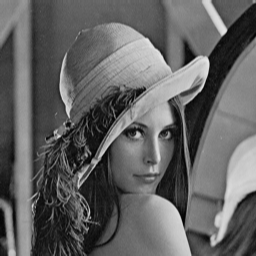
\includegraphics[width=\linewidth]{../results/lena_original}
			\captionof{figure}{Imagen original}
			\label{fig:lenaoriginal}
		\end{minipage}\hfill
		\begin{minipage}{0.45\linewidth}
			\centering
			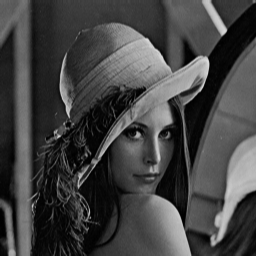
\includegraphics[width=\linewidth]{../results/lena_ej1}
			\captionof{figure}{Imagen modificada}
			\label{fig:lenaej1}
		\end{minipage}
	\end{frame}

	
	\begin{frame}{}
		\centering
		{\huge ¡Gracias!}\\
		\vspace{1cm}
		
\includegraphics[width=0.2\textwidth]{UNAHUR.png}
	\end{frame}
	
\end{document}
